\scanpage{48}
et sont ni égales, ni liées, ni opposées, i.e. ssi \inserted{$\tau\ne\tau'$ et} il existe une triade $\tau''$ liée à $\tau$ et $\tau'$.

\textcircled{\scriptsize 4} Soit $\tau$ une triade, soient $\tau',\tau''$ les deux triades liées à $\tau$. Alors
\[
\tau'\amalg\tau''=L(\tau)=\{\text{ens des }s\in S\smallsetminus\tau\text{ liés à aucun }\in\tau\}
\tag*{a)}
\]
\deleted{\unsure{a}} En particulier (compte tenu de \textcircled{\scriptsize 3}) $L(\tau)$ est une bitriade, et $L(\tau)=\tau'\cup\tau''$ est sa décomposition canonique
(ce qui explicite la construction des deux triades $\tau',\tau''$ contigues à une triade $\tau$)

\textcircled{\scriptsize 5} Soit $\bar\tau=E(\tau)$ l'ens des sommets liés à tous les él. de $\tau$. Alors $\bar\tau$ est une triade (donc la triade opposée à $\tau$).
D'où \textcircled{\scriptsize 6} Les deux triades biliées à $\tau$ s'obtient ainsi:
\[
\begin{aligned}
\text{l'une est}\quad&\overline{\tau'}=L(\tau'')\smallsetminus\tau\\
\text{l'autre}\quad&\overline{\tau''}=L(\tau')\smallsetminus\tau
\end{aligned}
\]
\deleted{\textcircled{\scriptsize 7} Les hexagones de triades}
\inserted{L'hexagone} de triades contenant $\tau$ est \deleted{\unsure{$\xi$}}
\[
\tau\ \tau'\ \overline{\tau''}\ \bar\tau\ \overline{\tau'}
\]
(si suivant dans cet ordre circulaire \ldots) \deleted{\unsure{donc}}. Aussi on trouve
\figure{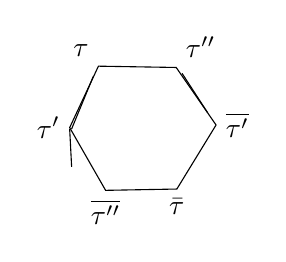
\begin{tikzpicture}[scale=.83]
\draw (-.68,1)--(.51,.98)--(1.12,.1)--(.52,-.88)--(-.57,-.9)--(-1.12,.06)--cycle;
\draw (-1.09,.04)--(-.76,.84) (.60,.89)--(.99,.29) (-1.12,.04)--(-1.09,-.54);
\node[above left] at (-.68,1) {$\tau$}; \node[above right] at (.51,.98) {$\tau''$};
\node[right] at (1.12,.1) {$\overline{\tau'}$}; \node[below] at (.52,-.88) {$\bar\tau$};
\node[below] at (-.57,-.9) {$\overline{\tau''}$}; \node[left] at (-1.12,.06) {$\tau'$};
\end{tikzpicture}}

\textcircled{\scriptsize 7} Pour la relation de ``biliées'', \deleted{\unsure{le graphe|les triades}} \inserted{l'ens} $\mathrm{Tri}$, \deleted{les triades} des triades est un graphe somme de triangles (dits \deleted{triangles triples} \inserted{``triangles} de triades biliées''), dans l'ens des triangles de triades biliées'' \deleted{\unsure{la rel.}} le passage au ``triangle opposé'' est une involution ss pt fixe.
% slanted
\margin{\unsure{Tritria|Tritrio} $={}$ triangle de triades biliées \deleted{est} de cardinal $2\cdot120=240$}
\inserted{les hexagones correspondent aux orbites de cette involution, à tt triangle correspond \unsure{la réunion|l'hexagone} de ce triangle et son opposé.}

\figure{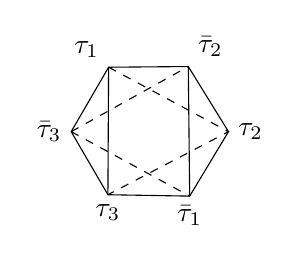
\begin{tikzpicture}[scale=.88]
\draw (-.62,.95)--(.53,.96)--(1.11,.02)--(.55,-.91)--(-.63,-.89)--(-1.16,.02)--cycle;
\draw (-.62,.95)--(-.63,-.89) (.53,.96)--(.55,-.91);
\draw[dashed] (-.62,.95)--(1.11,.02)--(-.63,-.89) (-1.16,.02)--(.53,.96) (-1.16,.02)--(.55,-.91);
\node[above left] at (-.62,.95) {$\tau_1$};\node[above right] at (.53,.96) {$\bar\tau_2$};
\node[right] at (1.11,.02) {$\tau_2$};\node[below] at (.55,-.91) {$\bar\tau_1$};
\node[below] at (-.63,-.89) {$\tau_3$};\node[left] at (-1.16,.02) {$\bar\tau_3$};
\end{tikzpicture}}
\deleted{\textcircled{\scriptsize 8} La réunion (de cardinal $6\cdot3=18$) des triades d'un hexagone a un complémentaire (de cardinal $27-18=9$) qui est un bitriangle. L'application qui à tt hexagone de triades associe \unsure{le} bitriangle précédent, est \uline{bijective}.}
\deleted{les Hexagones \unsure{correspondent}}
% archive sheet number: 47
